\newcommand{\highlightbox}[2]{%
    \colorbox{cyan!20}{%
        \parbox{#1}{\vspace{0.5em}\centering #2\vspace{0.5em}}%
    }%
}

\lstdefinelanguage{Pseudo}{
	keywords={FUNKTION, WENN, SOLANGE, DANN, FUER, JEDEN, JEDE ,ENDE, NAECHSTE, NAECHSTER, VON, FUNCTION, IMPORT, END if, then, void},
	morecomment=[l]{//}
}

\chapter{Suchproblem und Suchalgorithmen}

Ein Agent muss für ein bestimmtes Ziel die richtige Auswahl an Aktionen treffen und vorausschauend planen. Der Prozess der Bestimmung der Abfolge von Aktionen wird als Suche bezeichnet und mithilfe von Suchalgorithmen, wie A$^*$, durchgeführt. Für diesen Prozess benötigt der Agent einen Raum mit Regeln und Informationen, der im Suchproblem definiert wird. Ein Suchalgorithmus sucht die richtige Auswahl an Aktionen, auch Aktions-Sequenz genannt, über einen Suchbaum, welcher über das Suchproblem definiert wird. Die Informationen des folgenden Kapitel basieren auf den wissenschaftlichen Arbeiten \autocite{RN2020}, \autocite{4082128} und \autocite{Felner2011}.

\section{Suchproblem}

Ein Suchproblem wird durch einen Satz möglicher Zustände, einen Ausgangszustand, Zielzustände, Aktionen, ein Übergangsmodell und Aktionskosten definiert. Die Zustände beschreiben die Umwelt des Agenten. Der Ausgangszustand $s$ gibt den Zustand an, von dem der Agent startet. Ein Agent verfolgt ein oder mehrere Ziele, die durch Zielzustände definiert werden.

\[
\highlightbox{0.9\textwidth}{$
    \begin{aligned}
			s = \{AtCover, GunLoaded, PlayerAlive\}
    \end{aligned}
$}
\]

Die Aktionen die ein Agent besitzt können in bestimmten Zuständen $ACTIONS(s)$ ausgeführt werden.

\[
\highlightbox{0.9\textwidth}{$
    \begin{aligned}
			ACTIONS(GunLoaded) &= \{Shoot\} \\
			ACTIONS(\lnot GunLoaded) &= \{Reload\}
    \end{aligned}
$}
\]

Ein Übergangsmodell $TRANSITION(s,a) = s^*$ beschreibt den resultierenden Zustand $s^*$ der durch Aktionen $a$ im derzeitigen Zustand $s$ resultiert.

\[
\highlightbox{0.9\textwidth}{$
    \begin{aligned}
			TRANSITIONS(GunLoaded, Shoot) &= \lnot PlayerAlive
    \end{aligned}
$}
\]

Durch eine Aktion-Kosten Funktion $ACTIONCOST(s,a,s^*)$ erhalten wir die Kosten einer Aktion $a$, welche in einem Zustand $s$ ausgeführt wird und in einen neuen Zustand $s^*$ resultieren.

Die Lösung für ein Suchproblem ist die Sequenz an Aktionen, also der Plan, der vom Ausgangszustand zum Zielzustand führen soll. Der gewählte Pfad sollte die geringsten Kosten unter allen möglichen Lösungen aufweisen und somit eine optimale Lösung darstellen. Der Satz an möglichen Zuständen kann dabei als Suchbaum modelliert werden.


\section{Suchbaum}

Ein Suchbaum ist eine Baumstruktur, die in der Informatik für das speichern von Daten benutzt wird. Die Struktur basiert auf einer Anordnung von Knoten, welche mit anderen Knoten durch Kanten verbunden sind. Diese Knoten speichern speichern, je nach Anwendung bestimmte Daten. Besitzt der Suchbau einen Wurzelknoten, von dem aus sämtliche anderen Knoten erreichbar sind oder der seinerseits von jedem anderen Knoten aus erreicht werden kann, so spricht man von auch von einem Wurzelbaum. Es gibt verschiedene Typen von Suchbäumen die sich in ihren Eigenschaften und Zwecken unterscheiden, wie z.B. Binäre Suchbäume oder AVL-Bäume. In Abbildung X wird ein Suchbaum dargestellt.

\subsection{Knoten eines Suchbaums}
Ein Knoten speichert dabei:
\begin{itemize}
	\item Einen Zustand, zu dem die Aktion des jeweiligen Knoten geführt hat
	\item Eine Aktion, die auf dem Eltern-Knoten ausgeführt wurde
	\item Einen Eltern-Knoten, auf dem die Aktion durchgeführt wurde und den jeweiligen Knoten generiert hat
	\item Die Pfad-Kosten, der die summierten Kosten vom Ausgangsknoten bis zum jeweiligen Knoten speichert
\end{itemize}

\subsection{Gerichtete und ungerichtete Suchbäume}

Die Kanten bestimmten ob der Suchbaum gerichtet oder ungerichtet ist. In einem ungerichteten Suchbaum sind die Kanten zwischen den Knoten bidirektional. Das bedeutet, dass eine Kante keine feste Richtung vorgibt. Verbindet eine Kante die Knoten A und B, so ist die Kante in beide Richtungen durchquerbar. Das heißt, man kann sowohl von A nach B als auch von B nach A navigieren. In einem ungerichteten Suchbaum kann jeder Knoten der Wurzelknoten sein. Bei einem gerichteten Suchbaum, verbindet eine Kante zwei Knoten, wobei eine klare Richtung von einem Knoten (Elternknoten) zu einem Knoten (Kindknoten) vorgibt. Das bedeutet, dass die Kante nur in eine Richtung durchquerbar ist: vom Elternknoten zum Kindknoten.

\subsection{Balancierte und unbalancierte Suchbäume}

Eine weitere Eigenschaft des Suchbaums ist die Balance. So kann ein Suchbaum balanciert oder unbalanciert sein. Dafür wird auf die Anordnung der Knoten beachtet, beziehungsweise die Höhe. Die Höhe ist dabei die maximale Anzahl von Kanten von seiner Wurzel zu einem Blatt. 

Ein balancierter Baum ist eine Baumstruktur, bei der die Höhe des Baumes so organisiert ist, dass Such-, Einfüge- und Löschoperationen von Knoten effizienter durchgeführt werden können. In einem solchen Baum sind die Knoten gleichmäßig verteilt, sodass die Baumhöhe nicht zu hoch wird. Der Höhenunterschied zwischen den linken und rechten Teilbäumen darf dabei $<= 1$ entsprechen. Ein unbalancierter Baum hat einen Höhenunterschied $> 1$.

\begin{figure}[h]
  \centering
  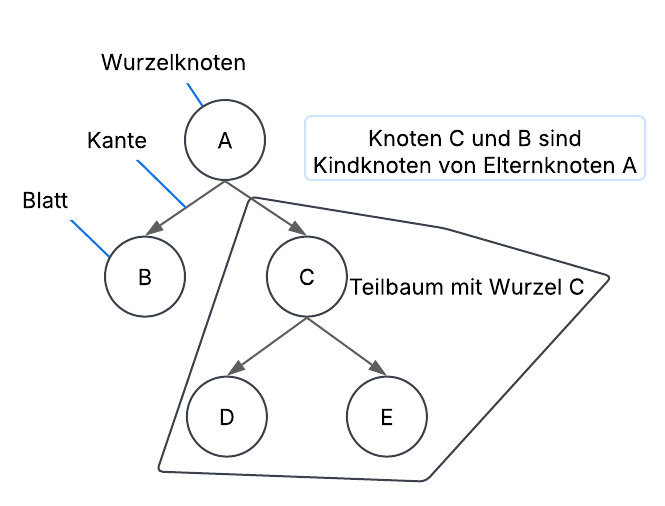
\includegraphics[width=10cm]{Suchalgorithmen/suchbaum_aufbau}
	\captionsetup{justification=justified, format=plain}
  \caption{Suchbaum Aufbau}
  \label{Suchalgorithmen}
\end{figure}

\section{Suchalgorithmen}

Das Suchproblem soll mit seinen Informationen durch einen Suchalgorithmus gelöst werden. Ein Suchalgorithmus sucht über einen Suchbaum einen Pfad zum Ziel. Wie effizient der gefundene Weg, hängt von dem Suchalgorithmus ab. So wird im Bereich der Suchalgorithmen wird zwischen informierten und uniformierten Algorithmen unterschieden. Informierte Algorithmen können dabei die Distanz zum Ziel über eine Heuristik schätzen, während uniformierte eine solche Schätzung nicht durchführen können.

Ein weiterer Unterschied ist die Zeit und Speicherkomplexität. Während uninformierte Algorithmen wie die Tiefensuche weniger Speicher benötigen, können sie ineffizient sein, da sie keine Richtung zum Ziel berücksichtigen. Informierte Algorithmen sind speicherintensiver, können aber Pfade schneller durch die Informationen der Heuristik finden.
Unter die uninformierten Suchalgorithmen fallen die Breitensuche, Dijkstra und Tiefensuche. Zu den informierten Suchalgorithmen gehören unter anderem die Bestensuchen: \textit{Greedy best-first-search} und der A* Algorithmus.


\subsection{Expansion einer Bestensuche}

Eine Bestensuche arbeitet sich schrittweise über Iterationen mithilfe von Expansionen zu einem Zielknoten vor. Vor der ersten Iteration wird ein Wurzelknoten mit dem Ausgangszustand generiert und einer offenen Liste hinzugefügt. Bei der offenen Liste handelt es sich um eine Vorrangwarteschlange (Priority Queue). So wird sichergestellt, dass bei der ersten Iteration der Wurzelknoten betrachtet wird.

In der Iteration werden Knoten der offenen Liste expandiert. Bei einer Expansion ermittelt der Algorithmus mithilfe der Funktion $TRANSITIONS(n)$ alle möglichen Kanten $ACTIONS(n)$, die vom aktuellen Knoten $n$ ausgehen und zu Kindknoten führen. Für die Kindknoten wird eine Bewertung durch die Bewertungsfunktion $f(n)$ berechnet, welche nach Suchalgorithmus variiert. Diese Kindknoten werden daraufhin sortiert nach ihrer Bewertung der offenen Liste hinzugefügt. Wenn ein Knoten expandiert wird, wird dieser aus der offenen Liste entfernt. Sollte der gelesene Knoten dem Ziel entsprechen, terminiert der Algorithmus und gibt den Knoten zurück. Ansonsten wird dieser expandiert und die resultierenden Kindknoten der offenen Liste hinzugefügt. Die Iteration wird solange fortgeführt bis der Zielknoten gefunden wurde oder sich keine Knoten in der offenen Liste befinden und somit keine Knoten zum Ziel führen.

Zu den Bestensuchen gehört unter anderem der \textit{Greedy best-first-search} und der A* Algorithmus, die sich in ihrer Bewertungsfunktion unterscheiden.

\lstinputlisting[firstline=0, language=Pseudo, linerange={31-55}, caption={Pseudocode Bestensuche}, label=lst:caption]{code/goap_agent.py}


\begin{figure}[h]
  \centering
  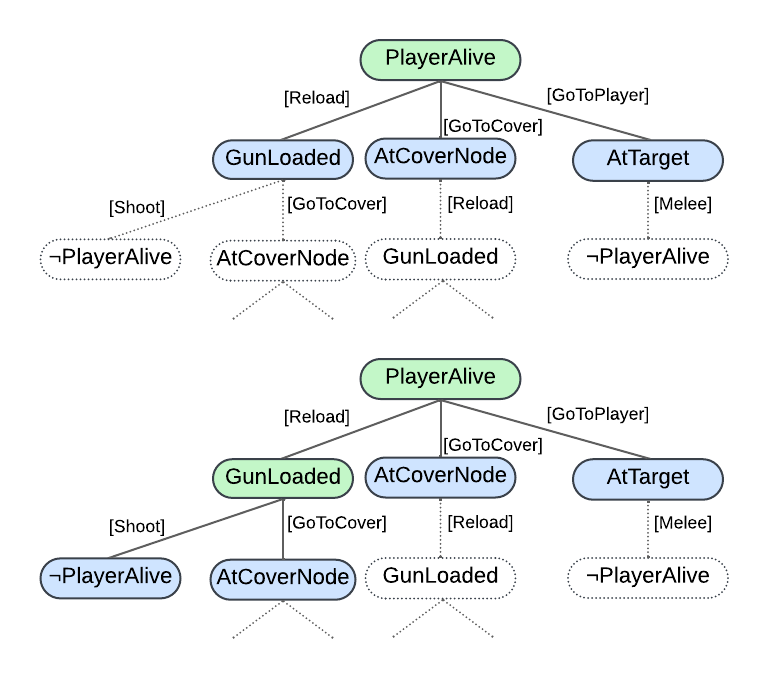
\includegraphics[width=15cm]{Suchalgorithmen/SAS}
	\captionsetup{justification=justified, format=plain}
  \caption{Suchbaum: Fängt vom Ausgangszustand an und soll den Zielzustand $\lnot \textit{PlayerAlive}$ erreichen. Grüne Knoten sind expandierte Knoten, welche in eine geschlossene Liste hinzugefügt werden. Blaue Knoten sind offene gefundene Nachbarknoten aus der offenen-Liste. Gestrichelte Knoten sind nicht entdeckte Knoten. Im Falle des Beispiels hat sich der Suchalgorithmus für den Knoten GunLoaded entschieden, da dieser optimaler als andere Nachbarknoten ist. Von dort aus ist der Zielzustand erreichbar und der Algorithmus würde eine Sequenz von Aktionen geben: \textit{[Reload,Shoot]}}
  \label{Suchalgorithmen}
\end{figure}
\clearpage

\subsection{A* Algorithmus}

Gehört zu den informierten und heuristischen Suchverfahren und ist eine Form der Bestensuche. Er ist ein vollständiger Algorithmus, was bedeutet, dass er einen Pfad zum Ziel und findet, wenn einer vorhanden ist. Der Einsatz des A* Algorithmus wird oft für Routenplaner benutzt. So benutzt Godot 4.3 den A* Algorithmus für die Navigation von NPC und GOAP, um eine optimale Sequenz an Aktionen zu finden, welche zum Zielzustand führt.

\subsubsection{Bewertungsfunktion}

Bestensuchen, wie A* benutzen eine Bewertungsfunktion $f(n)$, welche dazu dient die Priorität eines Knoten $n$ während der Suche zu bewerten. Bei der Bewertungsfunktion von A* werden dabei alle Pfad-Kosten $g(n)$ vom Ausgangsknoten bis zum Knoten $n$ mit der Heuristik $h(n)$ des Knoten $n$ summiert.

\[
\highlightbox{0.9\textwidth}{$
    \begin{aligned}
			f(n) = g(n) + h(n)
    \end{aligned}
$}
\]

Mit jeder Erweiterung des Pfades von $n$ zu $n^{\ast}$ steigen die Kosten $g(n)$. Dies liegt an den positiven tatsächlichen Aktion-Kosten $ACTIONCOST(n,a,n^*)$ der Kanten zwischen den Knoten.

\[
\highlightbox{0.9\textwidth}{$
    \begin{aligned}
			g(n) + ACTIONCOST(n,a,n^*) + h(n^*) &= g(n^*) + h(n^*)
    \end{aligned}
$}
\]

\subsubsection{Heuristik}

Ein Suchalgorithmus sollte einen Pfad mit möglichst geringen Kosten (optimalen-Pfad) zum Ziel finden. Ob A* einen optimalen Pfad findet, hängt von den Eigenschaften der Heuristik $h(n)$ ab. Eine Heuristik weist die Eigenschaften der Zulässigkeit und Konsistenz auf. Bei einer zulässigen Heuristik werden die Kosten stets unterschätzt oder genau geschätzt. Sie bleibt im Intervall $[0, h^{\ast}(n)]$ wobei $h^{\ast}(n)$ die tatsächlichen Kosten sind.

\[
\highlightbox{0.9\textwidth}{$
    \begin{aligned}
			0 \leq h(n) \leq h^*(n)
    \end{aligned}
$}
\]

Eine konsistente Heuristik, muss gleichzeitig zulässig sein und die Dreiecksungleichung erfüllen. Umgekehrt muss eine zulässige Heuristik nicht konsistent sein. So muss diese die Dreiecksungleichung erfüllen, welche besagt, dass die Heuristik $h(n)$ geringer sein soll als die Summe der Aktion $a$ und die Heuristik des folgenden Knoten $h(n^*)$.

\[
\highlightbox{0.9\textwidth}{$
    \begin{aligned}
			h(n) \leq ACTIONCOST(n,a,n^*) + h(n^*)
    \end{aligned}
$}
\]

Die konsistente Heuristik weist eine stärkere Eigenschaft auf als eine zulässige Heuristik. Der expandierte Knoten bei einer konsistenten Heuristik wird optimal sein, wodurch dieser Knoten nicht erneut in die offene-Liste hinzufügt werden muss.

Mit einer inkonsistenten Heuristik können Pfade auftreten, welche denselben Zustand erreichen. Somit können mehrere Pfade mit unterschiedlichen Kosten, aber demselben Zustand in der offenen Liste auftreten, was zur höheren Zeit. und Speicherkosten führt.

\subsubsection{Beweis für Optimalität}

Arbeitet der A* Algorithmus mit einer zulässigen oder konsistenten Heuristik, so wird diese den optimalen, kostengünstigsten Pfad zu einem Ziel finden.

Vorraussetzung:
\begin{itemize}
\item A* expandiert auf Knoten mit der geringsten $f(n)$
\item Wir haben zwei mögliche Zielknoten:
\begin{itemize}
	\item optimaler Zielknoten: $G_o$
	\item suboptimaler Zielknoten: $G_s_o$
\end{itemize}
\item Eine zulässige Heuristik: $0 \leq h(n) \leq h^*(n)$
\item Einen nicht expandierten Knoten: $n$
\end{itemize}

Beweis:
\begin{enumerate}
	\item Da keine weiteren Schritte vom Zielzustand möglich sind gilt: $h(G_o) \land h(G_s_o) = 0$
	\[
	\highlightbox{0.9\textwidth}{$
		\begin{align*}
			f(G_o) &= g(G_o) + h(G_o) \\
			f(G_o) &= g(G_o) \\
			f(G_s_o) &= g(G_s_o) + h(G_s_o) \\
			f(G_s_o) &= g(G_s_o)
		\end{align*}
	$}
	\]
	
	Da $G_s_$ suboptimal ist folgt, dass die Pfadkosten $f(n)$ von $G_s_o > G_o$ sind und somit: $f(G_s_o) > f(G_o)$.
	\item Da $g(G_o)$ der tatsächliche Zielknoten ist und $h^*(n)$ die tatsächlichen Kosten von $G_o$ sind gilt:
	\[
	\highlightbox{0.9\textwidth}{$
    \begin{align*}
			f(n) = g(n) + h(n) &< g(n) + h^*(n) = g(G_o) = f(G_o) \\
			f(n) &< g(G_o)
		\end{align*}
	$}
	\]
\end{enumerate}
Aus 1. und 2. folgt: $f(n) < f(G_o) < f(G_s_o)$. Somit würde A* nicht zu $G_s_o$ führen und ist mit einer zulässigen Heuristik optimal.

\begin{figure}[h]
  \centering
  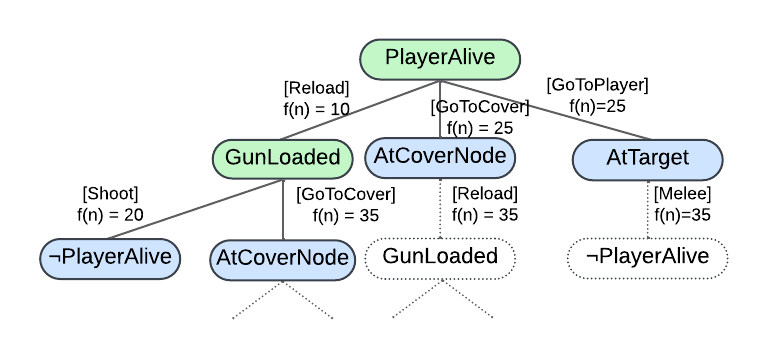
\includegraphics[width=15cm]{Suchalgorithmen/A_Erweiterung}
	\captionsetup{justification=justified, format=plain}
  \caption{A Suchalgorithmus: Der Pfad \textit{[Reload,Shoot]} hat mit $f(n)=20$ die geringsten Pfadkosten. Das Beispiel kommt aus  Abbildung 1.1. Wie genau $g(n)$ und $h(n)$ am Beispiel von NPC-Aktionen berechnet wird, wird im GOAP Kapitel erklärt.}
  \label{Suchalgorithmen}
\end{figure}